\section{Architecture}
This section describes the internal architecture of Spring XD. See figure~\ref{fig:architecture}.

\subsection{Application Context}
The foundation of Spring XD is the Spring application context. The application context is a dependency injection framework that is used to instantiate objects along with their dependencies \cite{spring-framework-reference}. 

\subsection{Modules}
A Spring XD Module is a unit of data processing. A stream processing module for Spring XD consists of one of three types: sources, processors, and sinks. A stream consists of a collection of modules that define a pipeline for data.

Modules in Spring XD are defined in their own application context. This allows for easy encapsulation and life cycle management for modules.

\subsection{Message Bus}
Modules require a data transport in order to transfer stream data. Spring XD supports pluggable transports via the Message Bus. Spring XD includes implementations based on Redis, RabbitMQ, and Kafka.

\begin{figure}[ht]
\centering
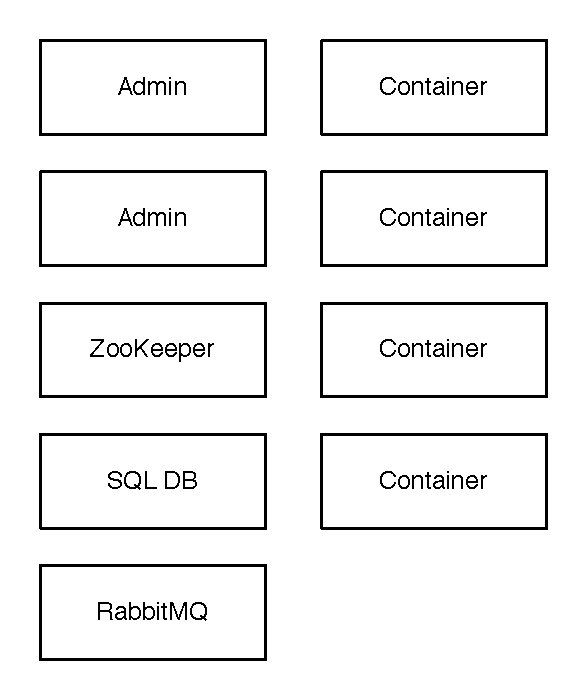
\epsfig{file=XD-sample.eps, height=2in, width=2in}
\caption{Spring XD Architecture.}
\label{fig:architecture}
\end{figure}

Here is where we get into the fine grained details.
